\chapter{Hart en longen tijdens inspanning}\label{ch:g10:heart-lungs-effort}

Ren vier trappen op en sta boven stil. Je borst gaat op en neer ---
veertig ademteugen per minuut in plaats van twaalf, elk drie keer zo diep
--- en je hart bonkt op honderdzeventig. Niets aan de trap vroeg je om
daartoe te besluiten; het lichaam regelde het in seconden, omdat de
spieren uit \cref{ch:g10:exercise-and-energy} tien keer meer zuurstof
eisten dan een minuut eerder. Dit hoofdstuk gaat over het
aanvoersysteem --- longen, hart, bloedvaten --- en over hoe zijn
opbrengst bij het begin van een inspanning wordt vermenigvuldigd.

\section{Ventilatie}

\begin{definition}[Ventilatie]\label{def:g10:heart-lungs-effort:ventilation}
De \emph{longventilatie}\index{ventilatie} is het luchtvolume dat per
minuut de longen in en uit gaat: het volume van één ademteug (het
\emph{ademvolume}) vermenigvuldigd met het aantal ademteugen per minuut
(de \emph{ademfrequentie}). In rust ongeveer \qty{0.5}{L}, twaalf tot
vijftien keer per minuut: \qtyrange{6}{8}{L/min}. In de longen bereikt de
lucht zo'n 300 miljoen \emph{longblaasjes}\index{longblaasje},
dunwandige zakjes omwikkeld met haarvaten, waar zuurstof in het bloed
overgaat en koolstofdioxide eruit.
\end{definition}

\begin{proposition}[Ventilatie tijdens inspanning]\label{prop:g10:heart-lungs-effort:vent-exercise}
Tijdens inspanning stijgen zowel het ademvolume als de frequentie: een
fitte volwassene kan \qty{2.5}{L} veertig keer per minuut ademen,
\qty{100}{L/min} of meer, vijftien keer de rustwaarde. De stijging begint
binnen de eerste seconden van de inspanning, nog vóór enige verandering
in het bloed, en komt uit op een niveau dat evenredig is met de zuurstof
die wordt verbruikt.
\end{proposition}
\admitted

\begin{omfigure}
\begin{tikzpicture}
\begin{axis}[
  width=0.9\linewidth, height=6.2cm,
  axis x line=bottom, axis y line=left,
  xmin=0, xmax=40, ymin=0, ymax=6.5,
  xlabel={tijd (s)}, ylabel={longvolume (L)},
  xlabel style={font=\small, at={(axis description cs:0.5,-0.1)}, anchor=north},
  ylabel style={font=\small},
  tick label style={font=\small}, xtick={0,10,20,30,40}, ytick={0,1,2,3,4,5,6},
  clip=false,
]
\addplot[thick, omDef, smooth, samples=200, domain=0:16]
  {2.7 + 0.25*sin(deg(2*pi*x/4))};
\addplot[thick, omDef] coordinates {(16,2.7) (18,2.95) (21,5.7) (25,5.7) (30,1.2) (33,1.2) (35,2.7)};
\addplot[thick, omDef, smooth, samples=100, domain=35:40]
  {2.7 + 0.25*sin(deg(2*pi*(x-35)/4))};
\draw[dashed, gray] (axis cs:0,1.2) -- (axis cs:40,1.2);
\draw[dashed, gray] (axis cs:0,5.7) -- (axis cs:40,5.7);
\draw[dashed, gray] (axis cs:0,2.45) -- (axis cs:18,2.45);
\draw[dashed, gray] (axis cs:0,2.95) -- (axis cs:18,2.95);
\draw[<->, omThm] (axis cs:38,1.2) -- (axis cs:38,5.7);
\node[font=\small, anchor=west, omThm] at (axis cs:38.4,3.5) {vitale};
\node[font=\small, anchor=west, omThm] at (axis cs:38.4,3.1) {capaciteit};
\draw[<->] (axis cs:8,2.45) -- (axis cs:8,2.95);
\node[font=\small, anchor=south] at (axis cs:8,3.0) {ademvolume, \qty{0.5}{L}};
\node[font=\small, anchor=north] at (axis cs:20,1.1) {restvolume};
\node[font=\small, anchor=south, align=center] at (axis cs:23,5.75) {maximale\\ inademing};
\node[font=\small, anchor=north, align=center] at (axis cs:31.5,1.1) {};
\end{axis}
\end{tikzpicture}

{\small Een spirogram: het luchtvolume in de longen tegen de tijd. Rustig
ademen verplaatst \qty{0.5}{L} per ademteug rond een middenstand; een
maximale inademing gevolgd door een maximale uitademing doorloopt de
vitale capaciteit, ongeveer \qty{4.5}{L}; de \qty{1.2}{L} die nooit kan
worden uitgedreven, is het restvolume.}
\end{omfigure}

\begin{example}[Een spirogram lezen]\label{ex:g10:heart-lungs-effort:spirogram}
In de figuur duren vier ademteugen \qty{16}{s}: 15 ademteugen per minuut
van \qty{0.5}{L}, dus \qty{7.5}{L/min}. De maximale uitslag loopt van
\qty{5.7}{L} tot \qty{1.2}{L}: een vitale capaciteit van \qty{4.5}{L}.
Een ademvolume van \qty{2.5}{L} tijdens inspanning gebruikt meer dan de
helft van die capaciteit, en daarom voelt zwaar ademen ook zo aan.
\end{example}

\begin{omfigure}
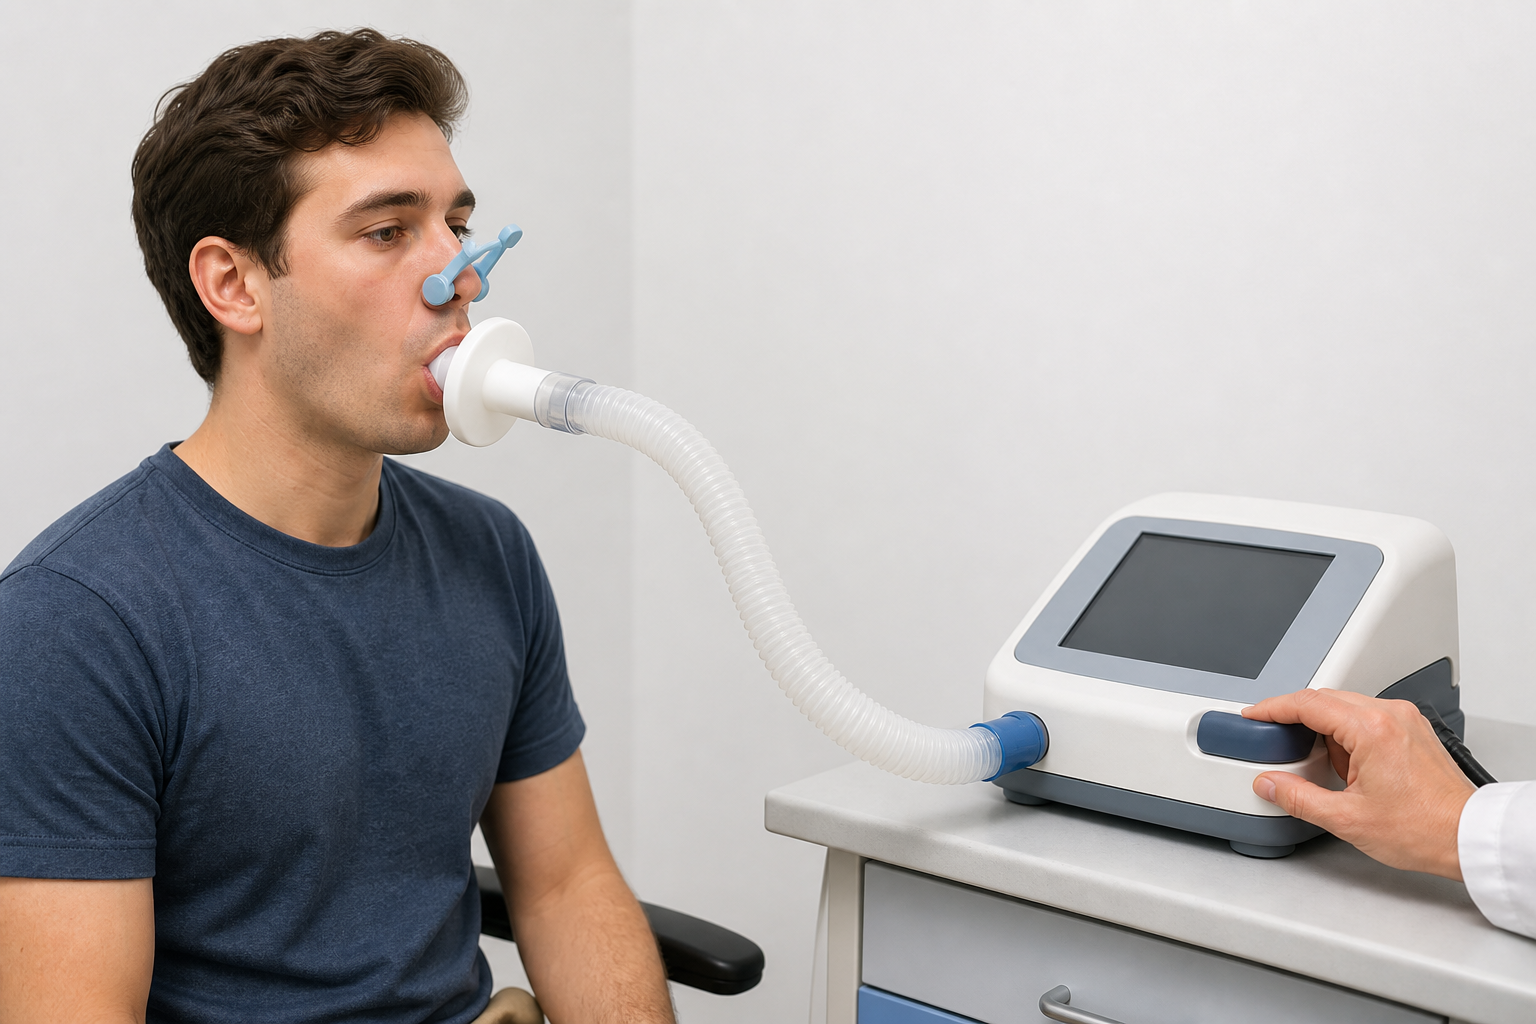
\includegraphics[width=0.58\linewidth]{images/book2/ai/g10-lungs-spirometer.png}

{\small Longvolumes meten: de proefpersoon ademt door een mondstuk in een
spirometer, met een klem op de neus, en het instrument legt het volume
van elke ademteug vast.}
\end{omfigure}

\section{Het hart en de twee bloedsomlopen}

\begin{definition}[Hartminuutvolume]\label{def:g10:heart-lungs-effort:output}
Het hart is een dubbele pomp met vier holten. De rechterkant ontvangt het
bloed dat van de organen terugkomt en stuurt het naar de longen (de
\emph{kleine bloedsomloop}); de linkerkant ontvangt het van de longen
terug en stuurt het naar de organen (de \emph{grote bloedsomloop}).
Kleppen tussen de holten en bij de uitgangen maken de stroom eenrichting.
Het \emph{hartminuutvolume}\index{hartminuutvolume} $Q$ is het volume
bloed dat elke kant per minuut pompt: het volume dat per slag wordt
uitgestoten, het \emph{slagvolume} $V_s$, vermenigvuldigd met de
\emph{hartfrequentie} $f$,
\[
Q = f \times V_s .
\]
In rust, $70$ slagen per minuut van \qty{70}{mL}: ongeveer
\qty{5}{L/min} --- het hele bloedvolume één keer per minuut.
\end{definition}

\begin{omfigure}
\begin{tikzpicture}[>=Stealth, font=\small,
  ch/.style={draw, thick, rounded corners, minimum width=1.9cm, minimum height=1.0cm, align=center},
  org/.style={draw, thick, rounded corners, minimum width=2.6cm, minimum height=1.0cm, align=center}]
  \node[org, fill=omDef!15] (lungs) at (3.5,3.6) {longen};
  \node[ch, fill=omDef!25] (ra) at (0.7,1.2) {rechter\\ boezem};
  \node[ch, fill=omDef!25] (rv) at (0.7,0) {rechter\\ kamer};
  \node[ch, fill=omThm!20] (la) at (6.3,1.2) {linker\\ boezem};
  \node[ch, fill=omThm!20] (lv) at (6.3,0) {linker\\ kamer};
  \node[org, fill=omThm!12] (org) at (3.5,-2.8) {spieren en\\ andere organen};
  \draw[->, thick, omDef] (ra) -- (rv);
  \draw[->, thick, omDef, rounded corners=6pt] (rv.west) -- (-1.55,0) -- (-1.55,3.6) -- (lungs.west);
  \node[anchor=east, align=right, omDef] at (-1.7,2.4) {long-\\ slagader};
  \draw[->, thick, omThm, rounded corners=6pt] (lungs.east) -- (8.6,3.6) -- (8.6,1.2) -- (la.east);
  \node[anchor=west, align=left, omThm] at (8.75,2.4) {long-\\ aderen};
  \draw[->, thick, omThm] (la) -- (lv);
  \draw[->, thick, omThm, rounded corners=6pt] (lv.east) -- (8.6,0) -- (8.6,-2.8) -- (org.east);
  \node[anchor=west, omThm] at (8.75,-1.4) {aorta};
  \draw[->, thick, omDef, rounded corners=6pt] (org.west) -- (-2.3,-2.8) -- (-2.3,1.2) -- (ra.west);
  \node[anchor=east, omDef] at (-2.45,-1.4) {aderen};
  \node[font=\small, anchor=north, text width=3.2cm, align=center] at (3.5,-3.6) {zuurstof eruit, $\mathrm{CO_2}$ erin};
  \node[font=\small, anchor=south, text width=3.2cm, align=center] at (3.5,4.2) {zuurstof erin, $\mathrm{CO_2}$ eruit};
  \draw[thick, dashed, gray] (3.5,2.5) -- (3.5,-1.9);
\end{tikzpicture}

{\small De dubbele bloedsomloop. Blauw: bloed dat arm is aan zuurstof,
door het rechterhart naar de longen gepompt. Rood: bloed dat rijk is aan
zuurstof, door het linkerhart naar de organen gepompt. De twee kanten
kloppen samen en pompen hetzelfde volume per minuut.}
\end{omfigure}

\begin{proposition}[Hartminuutvolume tijdens inspanning]\label{prop:g10:heart-lungs-effort:output-exercise}
Tijdens inspanning stijgt de hartfrequentie mee met het geleverde
vermogen, tot een maximum van ruwweg $220$ min de leeftijd in jaren, en
ook het slagvolume stijgt, bij een ongetraind mens met ongeveer de helft
en bij een getraind mens meer. Het \omterm{def:g10:heart-lungs-effort:output}{hartminuutvolume} van een jonge
volwassene gaat van \qty{5}{L/min} in rust naar
\qtyrange{20}{25}{L/min} bij maximale inspanning, en naar
\qty{35}{L/min} of meer bij een duursportkampioen, wiens slagvolume
\qty{180}{mL} kan overschrijden.
\end{proposition}
\admitted

\begin{omfigure}
\begin{tikzpicture}
\begin{axis}[
  width=0.86\linewidth, height=5.8cm,
  axis x line=bottom, axis y line=left,
  xmin=0, xmax=320, ymin=0, ymax=210,
  xlabel={mechanisch vermogen (W)}, ylabel={hartfrequentie (per min), slagvolume (mL)},
  xlabel style={font=\small, at={(axis description cs:0.5,-0.12)}, anchor=north},
  ylabel style={font=\small},
  tick label style={font=\small},
  xtick={0,50,100,150,200,250,300}, ytick={0,50,100,150,200},
  legend style={at={(0.5,-0.3)}, anchor=north, legend columns=3, font=\small, draw=none},
  clip=false,
]
\addplot[thick, omThm, mark=*, mark size=1.5pt] coordinates
  {(0,70) (50,95) (100,120) (150,145) (200,170) (250,190) (300,198)};
\addplot[thick, omDef, mark=square*, mark size=1.5pt] coordinates
  {(0,70) (50,90) (100,105) (150,112) (200,115) (250,115) (300,115)};
\addplot[thick, omMeth, dashed, mark=triangle*, mark size=1.8pt] coordinates
  {(0,4.9) (50,8.6) (100,12.6) (150,16.2) (200,19.6) (250,21.9) (300,22.8)};
\legend{hartfrequentie, slagvolume, minuutvolume (L/min)}
\end{axis}
\end{tikzpicture}

{\small Hartfrequentie, slagvolume en \omterm{def:g10:heart-lungs-effort:output}{hartminuutvolume} van een
twintigjarige bij toenemend vermogen. Het slagvolume vlakt bij matige
inspanning af; daarboven stijgt het minuutvolume alleen nog door de
frequentie, en die vlakt zelf af bij $220 - 20 = 200$.}
\end{omfigure}

\begin{example}[Minuutvolume bij \qty{200}{W}]\label{ex:g10:heart-lungs-effort:output200}
Uit de figuur: $f = 170$ per minuut, $V_s = \qty{115}{mL}$, dus
$Q = 170 \times 0.115 \approx \qty{19.6}{L/min}$: vier keer het
minuutvolume in rust. Het hart verplaatst het hele bloedvolume van het
lichaam vier keer per minuut.
\end{example}

\section{Het bloed brengen waar het nodig is}

\begin{proposition}[Herverdeling van de bloedstroom]\label{prop:g10:heart-lungs-effort:redistribution}
In rust ontvangen de spieren ongeveer een vijfde van het
\omterm{def:g10:heart-lungs-effort:output}{hartminuutvolume}; darm, lever en nieren nemen de helft. Bij zware
inspanning verwijden de kleine slagaders van de werkende spieren zich en
vernauwen die van de darm en de nieren: de spieren ontvangen dan meer dan
vier vijfde van een minuutvolume dat zelf is verviervoudigd --- zo'n
\qty{20}{L/min} in plaats van \qty{1}{L/min}, twintig keer meer. Het
aandeel van de hersenen blijft in absolute zin gelijk, en dat van de huid
stijgt om de warmte af te voeren.
\end{proposition}
\admitted

\begin{omfigure}
\begin{tikzpicture}
\begin{axis}[
  xbar stacked, bar width=15pt,
  width=0.86\linewidth, height=3.8cm,
  axis x line=bottom, axis y line=left,
  xmin=0, xmax=25, xlabel={bloedstroom (L/min)},
  xlabel style={font=\small, at={(axis description cs:0.5,-0.3)}, anchor=north},
  symbolic y coords={rust, maximale inspanning},
  ytick=data, tick label style={font=\small},
  enlarge y limits=0.5,
  legend style={at={(0.5,-0.65)}, anchor=north, legend columns=5, font=\small, draw=none},
]
\addplot[fill=omThm!50, draw=omThm] coordinates {(1.0,rust) (20.5,maximale inspanning)};
\addplot[fill=omProp!50, draw=omProp] coordinates {(2.5,rust) (0.9,maximale inspanning)};
\addplot[fill=omDef!50, draw=omDef] coordinates {(0.75,rust) (0.75,maximale inspanning)};
\addplot[fill=gray!40, draw=gray] coordinates {(0.5,rust) (1.2,maximale inspanning)};
\addplot[fill=omMeth!50, draw=omMeth] coordinates {(0.25,rust) (0.65,maximale inspanning)};
\legend{spieren, darm en nieren, hersenen, huid, overige}
\end{axis}
\end{tikzpicture}

{\small Waar het \omterm{def:g10:heart-lungs-effort:output}{hartminuutvolume} heen gaat, in rust (\qty{5}{L/min}) en
bij maximale inspanning (\qty{24}{L/min}). Het aandeel van de spieren
gaat van een vijfde naar meer dan vier vijfde; de hersenen houden hun
\qty{0.75}{L/min} onafgebroken.}
\end{omfigure}

\begin{proposition}[Aanvoer en onttrekking van zuurstof]\label{prop:g10:heart-lungs-effort:extraction}
Elke liter slagaderlijk bloed draagt ongeveer \qty{200}{mL} zuurstof,
vrijwel alles gebonden aan de hemoglobine van de rode bloedcellen. In
rust nemen de organen ongeveer \qty{50}{mL} uit elke liter; tijdens
inspanning nemen de werkende spieren er tot \qty{150}{mL} uit, drie keer
meer. De zuurstof die per minuut wordt verbruikt is het \omterm{def:g10:heart-lungs-effort:output}{hartminuutvolume}
vermenigvuldigd met de hoeveelheid die per liter wordt onttrokken --- dus
geven de vijfvoudige stijging van het minuutvolume en de drievoudige
stijging van de onttrekking samen de vijftienvoudige stijging van het
zuurstofverbruik uit \cref{ch:g10:exercise-and-energy}.
\end{proposition}
\admitted

\begin{example}[De zuurstofbalans getoetst]\label{ex:g10:heart-lungs-effort:fick}
Rust: \qty{5}{L/min} $\times$ \qty{50}{mL/L} $= \qty{250}{mL/min}$, het
verbruik in rust. Maximale inspanning van een getrainde leerling:
\qty{23}{L/min} $\times$ \qty{150}{mL/L} $= \qty{3.45}{L/min}$ --- een
$\dot V\!\mathrm{O_2}$max van \qty{50}{mL/min} per kilogram bij
\qty{69}{kg}, precies het cijfer van het vorige hoofdstuk.
\end{example}

\section{Hoe de reactie wordt geregeld}

\begin{proposition}[Zenuw- en hormoonregeling]\label{prop:g10:heart-lungs-effort:control}
Het hart en de ademhalingsspieren worden aangestuurd door zenuwcentra
onderin de hersenen. Twee stelsels zenuwen bereiken het hart: het ene
vertraagt het en is in rust actief; het andere versnelt het en versterkt
elke slag. Bij het begin van een inspanning wordt het bevel van de
hersenen aan de spieren naar die centra gekopieerd --- het hart versnelt
binnen één of twee slagen --- en sensoren in de spieren en gewrichten
melden de beweging. Naarmate de inspanning voortduurt, meten sensoren in
de slagaders vervolgens de koolstofdioxide en de zuurgraad van het bloed
en stellen zij de \omterm{def:g10:heart-lungs-effort:ventilation}{ventilatie} en de hartfrequentie zo bij dat die dicht
bij hun rustwaarden blijven. De bijnieren voegen het hormoon
\emph{adrenaline}\index{adrenaline} toe, dat de versnelling versterkt en
de slagaders van de spieren verwijdt.
\end{proposition}
\begin{proof}[Bewijsmateriaal]
De vertragende zenuw van een dier doorsnijden verhoogt zijn
rusthartfrequentie van 70 naar ongeveer 100; hem prikkelen legt het hart
stil. De versnellende zenuw prikkelen verdubbelt de frequentie. Iemand
die te horen krijgt dat er een inspanning aankomt, vertoont een stijgende
hartfrequentie nog vóór hij beweegt; een proefpersoon die lucht met extra
koolstofdioxide inademt, verhoogt zijn \omterm{def:g10:heart-lungs-effort:ventilation}{ventilatie} binnen een minuut, en
iemand bij wie de koolstofdioxide van het bloed tijdens de inspanning
kunstmatig constant wordt gehouden, verhoogt haar toch bij het begin van
de beweging --- de twee mechanismen, vooruitlopen en bijsturen, zijn
allebei echt.
\end{proof}

\begin{method}[De zuurstofaanvoer berekenen]\label{met:g10:heart-lungs-effort:compute}
\begin{enumerate}
  \item \omterm{def:g10:heart-lungs-effort:ventilation}{Ventilatie}: ademvolume $\times$ frequentie. Slechts ongeveer 70\%
        van elke ademteug bereikt de \omterm{def:g10:heart-lungs-effort:ventilation}{longblaasjes}; de rest vult de
        luchtwegen.
  \item \omterm{def:g10:heart-lungs-effort:output}{Hartminuutvolume}: $Q = f \times V_s$, in liter per minuut als
        $V_s$ in liter staat.
  \item Zuurstof die per minuut wordt verbruikt: $Q \times$ (zuurstof
        onttrokken per liter bloed).
  \item Stroom naar een orgaan: zijn aandeel in $Q$. Vergelijk absolute
        stromen, geen aandelen --- een kleiner aandeel van een groter
        minuutvolume kan meer bloed zijn.
  \item Toets: het verbruik kan niet boven de $\dot V\!\mathrm{O_2}$max
        uitkomen, en $f$ niet boven ongeveer $220 - $ de leeftijd.
\end{enumerate}
\end{method}

\begin{remark}[Waar de grens ligt]\label{rem:g10:heart-lungs-effort:limit}
De \omterm{def:g10:heart-lungs-effort:ventilation}{ventilatie} kan boven \qty{150}{L/min} komen en het bloed dat de longen
verlaat is bij maximale inspanning nog vrijwel verzadigd: de longen zijn
niet het knelpunt. Het slagvolume is dat wel: het bepaalt hoeveel bloed,
en dus hoeveel zuurstof, elke slag aanvoert. Duurtraining vergroot het
hart en zijn slagvolume --- en daarom klopt een getraind hart in rust op
45 in plaats van 70 voor dezelfde \qty{5}{L/min}, en daarom stijgt
$\dot V\!\mathrm{O_2}$max met training.
\end{remark}

\section{Oefeningen}

\begin{exercise}[$\star$]\label{exo:g10:heart-lungs-effort:1}
Bereken de \omterm{def:g10:heart-lungs-effort:ventilation}{ventilatie} van iemand die \qty{0.6}{L} veertien keer per
minuut ademt; en vervolgens die van dezelfde persoon die \qty{2.2}{L}
vijfendertig keer per minuut ademt.
\end{exercise}

\begin{exercise}[$\star$]\label{exo:g10:heart-lungs-effort:2}
Definieer het \omterm{def:g10:heart-lungs-effort:output}{hartminuutvolume} en geef de formule ervan. Bereken het voor
een hartfrequentie van 65 per minuut en een slagvolume van \qty{75}{mL}.
\end{exercise}

\begin{exercise}[$\star$]\label{exo:g10:heart-lungs-effort:3}
Volg de weg van een rode bloedcel van de rechterboezem terug naar de
rechterboezem, met de namen van de holten en de twee bloedsomlopen.
\end{exercise}

\begin{exercise}[$\star$]\label{exo:g10:heart-lungs-effort:4}
Geef uit de spirogramfiguur het ademvolume, de vitale capaciteit en het
restvolume.
\end{exercise}

\begin{exercise}[$\star$]\label{exo:g10:heart-lungs-effort:5}
Wat is de maximale hartfrequentie van een zestienjarige? En van een
zestigjarige?
\end{exercise}

\begin{exercise}[$\star\star$]\label{exo:g10:heart-lungs-effort:6}
Bereken uit de figuur van de hartfrequentie het \omterm{def:g10:heart-lungs-effort:output}{hartminuutvolume} bij
\qty{100}{W} en bij \qty{300}{W}, en de factor daartussen.
\end{exercise}

\begin{exercise}[$\star\star$]\label{exo:g10:heart-lungs-effort:7}
In rust ontvangen darm en nieren 50\% van \qty{5}{L/min}; bij maximale
inspanning 4\% van \qty{24}{L/min}. Bereken beide stromen. Wat verandert
sterker, het aandeel of de absolute stroom?
\end{exercise}

\begin{exercise}[$\star\star$]\label{exo:g10:heart-lungs-effort:8}
Een proefpersoon heeft een \omterm{def:g10:heart-lungs-effort:output}{hartminuutvolume} van \qty{18}{L/min} en haar
spieren onttrekken \qty{140}{mL} zuurstof per liter. Bereken haar
zuurstofverbruik. Zit zij dicht bij het plafond van een getrainde
leerling?
\end{exercise}

\begin{exercise}[$\star\star$]\label{exo:g10:heart-lungs-effort:9}
Waarom blijft de bloedstroom naar de hersenen op \qty{0.75}{L/min}
terwijl die naar de darm tijdens inspanning met twee derde wordt
teruggebracht? Denk aan wat elk orgaan kan verdragen.
\end{exercise}

\begin{exercise}[$\star\star$]\label{exo:g10:heart-lungs-effort:10}
Een getrainde wielrenster heeft een rusthartfrequentie van 42 en een
minuutvolume in rust van \qty{5}{L/min}. Bereken haar slagvolume en
vergelijk het met dat van een ongetraind mens.
\end{exercise}

\begin{exercise}[$\star\star$]\label{exo:g10:heart-lungs-effort:11}
Leg uit waarom de hartfrequentie al vóór de eerste pas van een wedstrijd
begint te stijgen, en wat er zou gebeuren met een loper wiens regeling
alleen op het meten van koolstofdioxide in het bloed werkte.
\end{exercise}

\begin{exercise}[$\star\star\star$]\label{exo:g10:heart-lungs-effort:12}
Twee proefpersonen bereiken dezelfde maximale hartfrequentie van 195. De
een heeft een maximaal slagvolume van \qty{110}{mL}, de ander
\qty{160}{mL}. Bereken bij dezelfde zuurstofonttrekking van
\qty{150}{mL/L} hun maximale zuurstofverbruik, en zeg wat
\cref{rem:g10:heart-lungs-effort:limit} over hun trainingsverleden
voorspelt.
\end{exercise}

\begin{exercise}[$\star\star\star$]\label{exo:g10:heart-lungs-effort:13}
Lucht bestaat voor 21\% uit zuurstof. Een proefpersoon ventileert bij
maximale inspanning \qty{100}{L/min} en verbruikt \qty{3.5}{L/min}
zuurstof. Welk deel van de ingeademde zuurstof gebruikt zij werkelijk?
Wat gebeurt er met de rest?
\end{exercise}

\begin{exercise}[$\star\star\star$]\label{exo:g10:heart-lungs-effort:14}
Een geneesmiddel blokkeert de versnellende zenuwen en de werking van
\omterm{prop:g10:heart-lungs-effort:control}{adrenaline} op het hart, en beperkt de hartfrequentie tot 110. Voorspel
het effect ervan op het \omterm{def:g10:heart-lungs-effort:output}{hartminuutvolume} bij maximale inspanning, op de
$\dot V\!\mathrm{O_2}$max, en op wat de patiënt kan doen.
\end{exercise}

\begin{exercise}[$\star\star\star$]\label{exo:g10:heart-lungs-effort:15}
Bij iemand op grote hoogte draagt het slagaderlijke bloed \qty{150}{mL}
zuurstof per liter in plaats van \num{200}. Bereken bij hetzelfde
maximale \omterm{def:g10:heart-lungs-effort:output}{hartminuutvolume} en dezelfde onttrekking van 75\% van de
aangevoerde zuurstof het verlies aan $\dot V\!\mathrm{O_2}$max in
procenten. Stel één aanpassing voor die het lichaam in de weken daarna
maakt.
\end{exercise}

\section{Probleem: De inspanningstest}

\begin{problem}[{Weekendprobleem --- een inspanningstest bij de
cardioloog: hartfrequentie, slagvolume, ventilatie en zuurstofonttrekking
gemeten bij oplopend vermogen, en de vermenigvuldiging die zij samen
bereiken}]
\label{pb:g10:heart-lungs-effort:1}
Tom, 17 jaar, massa \qty{68}{kg}, trapt op een laboratoriumfiets terwijl
zijn hartfrequentie, \omterm{def:g10:heart-lungs-effort:ventilation}{ventilatie} en uitgeademde lucht worden vastgelegd.
Uitkomsten:

\begin{center}
\begin{tabular}{lccccc}
vermogen (W) & 0 & 75 & 150 & 225 & 300 \\ \hline
hartfrequentie (per min) & 62 & 105 & 140 & 175 & 198 \\
slagvolume (mL) & 72 & 100 & 116 & 120 & 120 \\
ademvolume (L) & 0.5 & 1.2 & 1.8 & 2.3 & 2.6 \\
ademteugen per min & 13 & 18 & 24 & 32 & 44 \\
$\mathrm{O_2}$ onttrokken per liter bloed (mL) & 52 & 90 & 120 & 145 & 155 \\
\end{tabular}
\end{center}

\medskip
\noindent\textbf{Deel I --- Het hart.}
\begin{enumerate}
  \item Bereken het \omterm{def:g10:heart-lungs-effort:output}{hartminuutvolume} van Tom bij elk vermogen.
  \item Met welke factor is het minuutvolume bij \qty{300}{W} gestegen?
        Welk deel van die factor komt van de frequentie en welk deel van
        het slagvolume?
  \item Boven welk vermogen houdt het slagvolume op te stijgen? Wat
        verhoogt het minuutvolume daarboven nog als enige?
  \item Vergelijk de maximale hartfrequentie van Tom met de vuistregel.
  \item Zijn minuutvolume in rust is ongeveer \qty{4.5}{L/min}. Als zijn
        bloedvolume \qty{5}{L} is, hoelang duurt één volledige rondgang
        in rust, en bij \qty{300}{W}?
\end{enumerate}

\medskip
\noindent\textbf{Deel II --- De longen.}
\begin{enumerate}[resume]
  \item Bereken de \omterm{def:g10:heart-lungs-effort:ventilation}{ventilatie} bij elk vermogen.
  \item Met welke factor is zij bij \qty{300}{W} gestegen? Welke van de
        twee factoren, volume of frequentie, draagt meer bij?
  \item De vitale capaciteit van Tom is \qty{5.0}{L}. Welk deel daarvan
        gebruikt elke ademteug bij \qty{300}{W}?
  \item De \omterm{def:g10:heart-lungs-effort:ventilation}{ventilatie} steeg met een grotere factor dan het
        \omterm{def:g10:heart-lungs-effort:output}{hartminuutvolume}. Betekent dat dat de longen de prestatie
        begrenzen? Gebruik \cref{rem:g10:heart-lungs-effort:limit}.
  \item Slechts 70\% van elke ademteug bereikt de \omterm{def:g10:heart-lungs-effort:ventilation}{longblaasjes}. Bereken
        de alveolaire \omterm{def:g10:heart-lungs-effort:ventilation}{ventilatie} in rust en bij \qty{300}{W}.
\end{enumerate}

\medskip
\noindent\textbf{Deel III --- De zuurstof.}
\begin{enumerate}[resume]
  \item Bereken het zuurstofverbruik van Tom bij elk vermogen, uit het
        \omterm{def:g10:heart-lungs-effort:output}{hartminuutvolume} en de zuurstof die per liter wordt onttrokken.
  \item Druk de waarde bij \qty{300}{W} uit in milliliter per minuut per
        kilogram. Is dat een $\dot V\!\mathrm{O_2}$max, en van wat voor
        proefpersoon?
  \item Met welke factor is het verbruik van rust tot \qty{300}{W}
        gestegen? Splits die op in de factor van het hart en de factor van
        de onttrekking.
  \item Bereken met \qty{20}{kJ} per liter zuurstof het metabole vermogen
        bij \qty{300}{W} en het rendement van de spieren (mechanisch
        vermogen gedeeld door het metabole vermogen boven de rust).
  \item Teken, of beschrijf, het zuurstofverbruik tegen het mechanische
        vermogen. Is het recht? Waar ligt het plafond?
\end{enumerate}

\medskip
\noindent\textbf{Deel IV --- De regeling en het oordeel.}
\begin{enumerate}[resume]
  \item De hartfrequentie van Tom kwam op 75 terwijl hij zat te wachten
        tot de test begon. Verklaar dat.
  \item Bij \qty{300}{W} is zijn slagaderlijke bloed nog voor 95\% met
        zuurstof verzadigd. Wat zegt dat over de uitwisseling in de
        \omterm{def:g10:heart-lungs-effort:ventilation}{longblaasjes}, en over waar de grens van zijn
        $\dot V\!\mathrm{O_2}$max ligt?
  \item De cardioloog merkt op dat de spieren nu ongeveer
        \qty{20}{L/min} bloed ontvangen. Welk deel van het minuutvolume
        is dat, en waar is de rest van de verdeling in rust gebleven?
  \item Na zes maanden training is het maximale slagvolume van Tom
        \qty{140}{mL} bij dezelfde maximale frequentie en onttrekking.
        Bereken zijn nieuwe $\dot V\!\mathrm{O_2}$max.
  \item Geef het resultaat: de drie getallen (hart, onttrekking,
        \omterm{def:g10:heart-lungs-effort:ventilation}{ventilatie}) waarmee het lichaam van Tom zijn zuurstofaanvoer in
        rust vermenigvuldigde, en welk daarvan de training veranderde.
\end{enumerate}
\end{problem}
